
\documentclass[
	12pt,
	openright,
	a4paper,
	english,			
	french,				
	spanish,			
	brazil,				
	]{abntex2}



\usepackage{lmodern}			
\usepackage[T1]{fontenc}		
\usepackage[utf8]{inputenc}		
\usepackage{indentfirst}		
\usepackage{color}				
\usepackage{graphicx}			
\usepackage{microtype} 			
\usepackage{multicol}
\usepackage{multirow}

\usepackage{float}
\usepackage{pdflscape}
\usepackage{rotating}

\usepackage{xcolor}
\definecolor{verde}{rgb}{0,0.5,0}
\usepackage{listings}
\lstset{
  language=Verilog,
  basicstyle=\ttfamily\tiny, 
  keywordstyle=\color{blue}, 
  stringstyle=\color{verde}, 
  commentstyle=\color{gray}, 
  extendedchars=true, 
  showspaces=false, 
  showstringspaces=false, 
  numbers=left,
  numberstyle=\tiny,
  breaklines=true, 
  backgroundcolor=\color{green!10},
  breakautoindent=true, 
  captionpos=b,
  xleftmargin=0pt,
}

\usepackage[brazilian,hyperpageref]{backref}	
\usepackage[num]{abntex2cite}	
\citebrackets() 


\renewcommand{\backrefpagesname}{Citado na(s) página(s):~}
\renewcommand{\backref}{}
\renewcommand*{\backrefalt}[4]{
	\ifcase #1 
		Nenhuma citação no texto.
	\or
		Citado na página #2.
	\else
		Citado #1 vezes nas páginas #2.
	\fi}


\titulo{Laboratório de Arquitetura e Organização de
Computadores: CoreBassier }
\autor{Leonardo Courbassier Martins} 
\local{São José dos Campos - Brasil}
\data{Julho de 2018}
\instituicao{
  Docente: Prof. Dr. Sérgio Ronaldo
  \par
  Universidade Federal de São Paulo - UNIFESP
  \par
  Instituto de Ciência e Tecnologia - Campus São José dos Campos
}
\tipotrabalho{Relatório técnico}
\preambulo{Relatório apresentado à Universidade Federal de São Paulo como parte dos requisitos para aprovação na disciplina de Laboratório de Sistemas Computacionais: Arquitetura e Organização de Computadores.}


\definecolor{blue}{RGB}{41,5,195}

\makeatletter
\hypersetup{
		pdftitle={\@title}, 
		pdfauthor={\@author},
    	pdfsubject={\imprimirpreambulo},
	    pdfcreator={LaTeX with abnTeX2},
		pdfkeywords={abnt}{latex}{abntex}{abntex2}{relatório técnico}, 
		colorlinks=true,       		
    	linkcolor=blue,          	
    	citecolor=blue,        		
    	filecolor=magenta,      		
		urlcolor=blue,
		bookmarksdepth=4
}
\makeatother


\setlength{\parindent}{1.3cm}
\setlength{\parskip}{0.2cm}
\makeindex

\begin{document}

\selectlanguage{brazil}

\frenchspacing 

\imprimircapa
\imprimirfolhaderosto*

%\setlength{\absparsep}{18pt} % ajusta o espaçamento dos parágrafos do resumo
%\begin{resumo}
%Este relatório tem como objetivo mostrar a implementação de um processador, desde seu \textit{design} até 
%até seu teste em um dispositivo FPGA.\\\\
% \noindent
% \textbf{Palavras-chaves}: arquitetura. processador. FPGA.
%\end{resumo}

\pdfbookmark[0]{\listfigurename}{lof}
\listoffigures*
\clearpage

\pdfbookmark[0]{\listtablename}{lot}
\listoftables*
\clearpage

\pdfbookmark[0]{\contentsname}{toc}
\tableofcontents*


\textual

\chapter{Introdução}
A arquitetura e a organização de um computador é fundamental e 
única em cada sistema que existe. A partir deles, é possível 
comparar diferentes processadores e sabendo a filosofia de 
cada um deles, é possível escolher um que mais se adequa a um
 determinado projeto.\\
É indiscutível que o processador é uma das partes mais 
importantes de um computador e, por isso, deve ser projetada 
com cautela e com técnicas cada vez mais aprimoradas para 
construir processadores cada vez mais rápidos e completos.\\
A mudança do tamanho de computadores é um bom exemplo de 
como uma boa organização do computador pode fazer diferença; 
E é necessário, cada vez mais, um desenvolvimento de 
ténicas para uma tecnologia cada vez mais avançada.\\
Atualmente, com o crescimento da Internet das Coisas, as diferentes topologias
emergentes têm processadores. Isso só reforça o quão importante
esse componente computacional é. Com isso, saber projetar um processador
para devidos tipos de problemas é fundamental na computação.\\

\chapter[Objetivos]{Objetivos}
\section{Geral}
O objetivo desse projeto é desenvolver um processador e testá-lo na 
placa FPGA. O processador deve ser capaz de rodar qualquer algoritmo já visto nas disciplinas
anteriores.

\section{Específico}
Descrição da arquitetura do processador e do conjunto de instruções; 
Desenvolvimento e implementação da ULA (Unidade Lógica Aritmética), 
Banco de Registradores, Memória de Dados, módulo Contador de Programa, 
Unidade de Controle e módulo de Entrada e Saída.

\chapter{Fundamentação Teórica}
\section{Processador}
O processador é uma parte de um sistema computacional, que utiliza de um conjunto de instruções para executar a aritmética básica, lógica, e a entrada e saída de dados. O processador tem um papel parecido ao cérebro no computador, pois ele controla todo os periféricos do computador e é o núcleo dele.\\
Além de saber o para quê serve, uma pergunta mais interessante é: Como funciona um processador?\\
Como é feita a implementação de um processador? Além dessas perguntas, é necessário conhecer o público-alvo do processador. O processador será projetado para programadores (dando várias instruções diferentes e diversas opções) ou será projetado para usuários comuns?
A resposta para essas perguntas dividem o processador em várias técnicas de \textit{design}.\\
As suas implementações vem mudando drásticamente desde o primeiro processador (Intel 4004, em 1971), assim como a tecnologia também vem desenvolvendo-se, surgiram diversas arquiteturas, organizações, entre outros. Já foram testados várias combinações de organizações até a que compreende-se como a melhor atualmente.

\section{Arquitetura}
Dentre os diversos tipos de arquitetura existentes, as mais conhecidas são as arquiteturas RISC (\textit{Reduced Instruction Set Computer}) e CISC (\textit{Complex Instruction Set Computer}).\\
A estratégia de \textit{design} RISC foca-se em um número pequeno de instruções, diminuindo o CPI (\textit{Clock per Instruction}) e a complexidade do processador.\\
Em contrapartida, a estratégia CISC foca-se em um número grande de instruções, o que facilita muito a programação, com várias instruções complexas, e com isso, a complexidade dos programas feitos em máquinas CISC são menores (em relação ao número de instruções).
Geralmente, as instruções tem um maior CPI, mas isso é compensado com uma funcionalidade não trivial.
Foi escolhido o modelo de arquitetura RISC para este relatório.\\

\section{MIPS}
Como referência de processador, foi utilizado o MIPS. O MIPS é um estilo de processador que não tem um único processador físico. 
\\
Quando foi comercializado em 1981, era comercializado a ideia do processador e outras empresas faziam a implementação delas. Sua característica principal é ser muito simples e didático e ele foi um grande influenciador das próximas arquiteturas RISC.\\
A sua implementação com \textit{pipeline} é bem rápida e não é tão complexa, e seus programas não ficam muito complexos.\\
O MIPS contém 32 registradores em sua implementação e alguns deles são reservados para o sistema. Além disso ele possui uma unidade de controle que facilita todo o controle do processador e seus componentes.\\

\subsection{Arquitetura do MIPS}
Na \autoref{fig:esquematico}, vemos o esquemático da arquitetura MIPS.\\
Como o MIPS é RISC, vemos que sua arquitetura é simples de ser entendida. Cada módulo na figura tem um papel específico, como descrito a seguir:\\
O módulo do PC tem a função de atualizar o Contador de Programa para buscar a próxima instrução do programa atual. Esse endereço entra no módulo da memória de Instruções, onde a próxima
instrução é buscada. A instrução atual é decodificada então, e as \emph{flags} são definidas pela Unidade de Controle. Os operadores da instrução são carregados do Banco de Registradores 
e as entradas corretas são enviadas para a Unidade Lógica e Aritmética para realizar a operação explicitado pela instrução. O resultado da ALU é escrito no Banco de Registradores ou na Memória de Dados, de acordo com a instrução atual. 
Após isso o valor do PC é atualizado e o ciclo continua.\\


\begin{figure}[H]
\centering 
\caption{Esquematico do MIPS} \label{fig:esquematico}
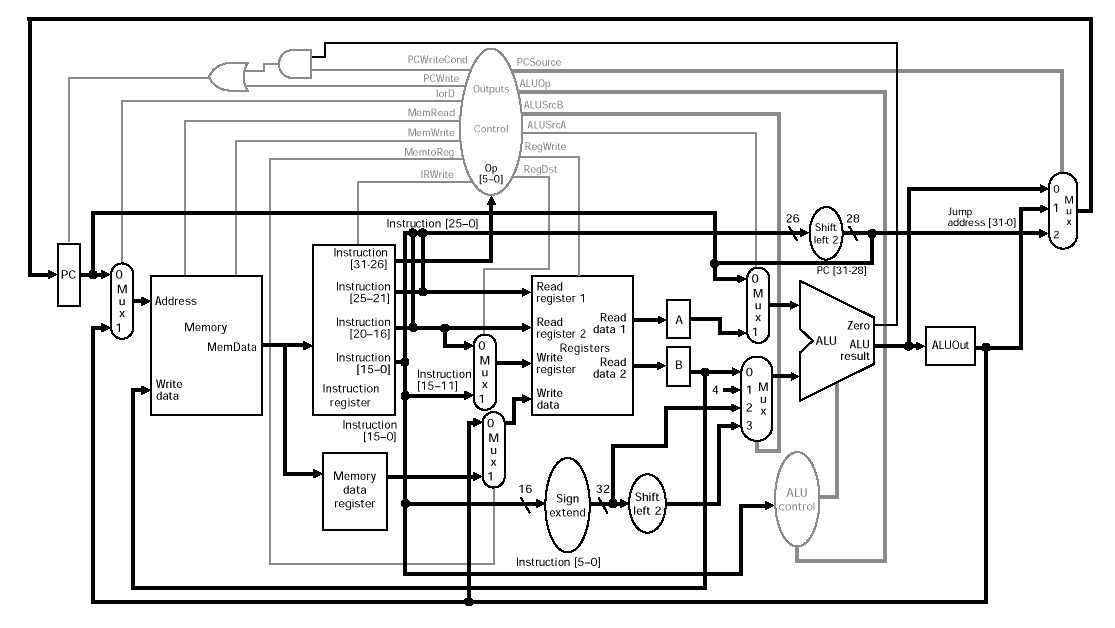
\includegraphics[scale=0.3]{esquematico.png}
\legend{Fonte: Computer Organization and Design \cite{patterson2007} }
\end{figure}

\subsection{Tipos de Instrução}
O MIPS possui três tipos de instruções que são caracterizados como: Tipo R, que é ilustrado na \autoref{tab:Instr3OP}:
\begin{table}[htb]
\centering
\ABNTEXfontereduzida
\caption{Formato das Instruções do Tipo R} \label{tab:Instr3OP}
\begin{tabular}{r|p{2cm}|p{1.7cm}|p{1.7cm}|p{1.7cm}|p{1.7cm}|p{3cm}} 
\textbf{Campo} & OpCode & RS & RT & RD & Shamt & Funct \\ \hline
\textbf{Tamanho (bits)} & 6 & 5 & 5 & 5 & 5 & 6 \\ \hline
\end{tabular}
\legend{Fonte: O Autor}
\end{table}

E a seguir são descritas as instruções do tipo R: add,
addu, 	
and,	
div, 	
jr,
mfhi, 	
mflo, 	
mfc0, 	
mult, 	
xor, 	 	
or, 	
sltu, 	
sll, 	
sra, 	
sub.

Além do tipo R, existe o tipo I que é ilustrado na \autoref{tab:Instr3OP2}


\begin{table}[htb]
\centering
\ABNTEXfontereduzida
\caption{Formato das Instruções do Tipo I} \label{tab:Instr3OP2}
\begin{tabular}{r|p{2cm}|p{1.7cm}|p{1.7cm}|p{3cm}} 
\textbf{Campo} & OpCode & RS & RT & Im \\ \hline
\textbf{Tamanho (bits)} & 6 & 5 & 5 & 16\\ \hline
\end{tabular}
\legend{Fonte: O Autor}
\end{table}

São instruções do tipo I as seguintes: 
addi,
addiu, 
andi,
beq,
blez,
bne,
lbu,
lhu,
lui,
lw,	
ori,
sb,
sh,		
slti, 	
sltiu,
sw.

Por último, existe o tipo J que é ilustrado na \autoref{tab:Instr3OP3}
\begin{table}[htb]
\centering
\ABNTEXfontereduzida
\caption{Formato das Instruções do Tipo J} \label{tab:Instr3OP3}
\begin{tabular}{r|p{2cm}|p{1.7cm}|p{1.7cm}|p{3cm}} 
\textbf{Campo} & OpCode & Address \\ \hline
\textbf{Tamanho (bits)} & 6 & 26\\ \hline
\end{tabular}
\legend{Fonte: O Autor}
\end{table}

São instruções do tipo J as seguintes: j, jal.

\subsection{Modos de endereçamento}
Descritas mais profundamente no \cite{patterson2007} e, brevemente em \cite{addrmodes}, o MIPS tem vários modos de endereçamento e são utilizados em diferentes instruções.\\
Abaixo está descrito os modos de endereçamento do MIPS, qual seu uso e como funciona.
\begin{itemize}
	\item Endereçamento por registrador: É utilizado esse modo de endereçamento quando os operandos estão em registradores, p.e. add;
	\item Endereçamento por imediato: É utilizado quando deve-se somar o valor de um registrador com um número definido como imediato, p.e. addi;
	\item Endereçamento de base-deslocamento: É utilizado quando o operando é soma de um imediato com um registrador, p.e. lw;
	\item Endereçamento relativo ao PC: É utilizado quando o dado é a soma do imediato com a posição atual do PC, p.e. beq;
	\item Endereçamento absoluto: É utilizado quando o dado é passado diretamente pela instrução, p.e. j;
\end{itemize}

\chapter{Desenvolvimento}
Essa seção mostra os pontos principais da implementação do processador. O processador aqui aprensetado é monociclo, sem \textit{pipeline} e RISC. Contém 28 instruções (discutidas nas próximas seções) e 5 tipos de formatos de instruções.\\
Além disso, ele possui 32 registradores de 32 bits, mas apenas alguns de próposito geral.

\section{Formato das Instruções}
Antes da implementação do processador, é necessário definir os formatos de instruções que será utilizado. A \autoref{tab:Instr3OP4} contém todos os 5 formatos, divindo os bits e os campos de cada formato.
\begin{table}[htb]
\centering
\ABNTEXfontereduzida
\caption{Formato das Instruções do CoreBassier} \label{tab:Instr3OP4}
\begin{tabular}{cl} 
	\textbf{Tipo} & \textbf{Campos}\\
	1 & [ OpCode / RegDest / RegOrigem / RegAlvo /\ | ]\\
	  &  \ \ [31:26]\ \ \ \ \ \ [25:21]\ \ \ \ \ \ \ \ [20:16]\ \ \ \ \ \ \ \ [15:11]\ \ \ [10:0]\\
	\hline
	\\
	2 & [ OpCode / RegDest / RegOrigem / Imediato (ou |) ]\\
	  &  \ \ [31:26]\ \ \ \ \ \ [25:21]\ \ \ \ \ \ \ \ [20:16]\ \ \ \ \ \ \ \ \ \ \ [15:0]\\
	\hline
	\\
	3 & [ OpCode / RegDest / RegOrigem (ou |) / Imediato (ou |) ]\\
	  &  \ \ [31:26]\ \ \ \ \ \ [25:21]\ \ \ \ \ \ \ \ \ \ \ [20:16]\ \ \ \ \ \ \ \ \ \ \ \ \ \ \ \ \ \ \ \ [15:0]\\
	\hline
	\\
	4 & [ OpCode / RegDest / Imediato ]\\
	  &  \ \ [31:26]\ \ \ \ \ \ [25:21]\ \ \ \ \ \ \ \ [20:0]\\
	\hline
	\\
	5 & [ OpCode / RegDest (ou |) / EndereçoAlvo (ou |) ]\\
	  &  \ \ [31:26]\ \ \ \ \ \ [25:21]\ \ \ \ \ \ \ \ \ \ \ \ \ \ [20:16]\\
	\hline
\end{tabular}
\legend{Fonte: O Autor}
\end{table}
  
O tipo 1 destina-se a operações aritméticas com três registradores e sem imediato. Já o tipo 2, destina-se a operações aritméticas com dois registradores e um imediato. O tipo 3, destina-se aos desvios de fluxos condicionais e incondicionais. O tipo 4, destina-se as instruções de entrada e saída, comunicação que será desenvolvida mais adiante (mais sobre isso nos próximos tópicos). Já o tipo 5, destina-se as instruções de controle do processador.\\
É fácil perceber que o formato das instruções aqui ilustrados para o CoreBassier é muito semelhante aos formatos do MIPS.\\
A maior diferença entre os dois processadores é que o MIPS utiliza do Shamt e Funct para as instruções e o outro não, foram criados mais formatos de instruções para deixar mais modular e mais simples de se entender.

\section{Conjunto de Instruções}
A \autoref{tab:Instr3OP5} contém todo o conjunto de instruções que o processador terá, os tipos das instruções e seu opCode.

\begin{table}[htb]
\centering
\ABNTEXfontereduzida
\caption{Conjunto de Instruções do CoreBassier} \label{tab:Instr3OP5}
\begin{tabular}{ ccc }
 	\textbf{OpCode} & \textbf{Instrução} & \textbf{Tipo}\\
 	000000 & Add & 1\\
 	000001 & Addi & 2\\
 	000010 & Sub  & 1\\
 	000011 & Subi & 2\\
 	000100 & Mult & 1\\
 	000101 & Multi & 2\\
 	000110 & Div & 1\\
 	000111 & Divi & 2\\
 	001000 & Mod & 1\\
 	001001 & Slt & 1\\	
 	001010 & Slti & 2\\
 	001011 & And & 1\\
 	001100 & Andi & 2\\
 	001101 & Or & 1\\
 	001110 & Ori & 2\\
 	001111 & Not & 2\\
 	010000 & ShR & 2\\
 	010001 & ShL & 2\\
 	010010 & Sgt & 1\\
 	010011 & Sgti & 2\\
 	010100 & Load & 4\\
 	010101 & Store & 4\\
 	010110 & Jump & 3\\
 	010111 & Beq & 3\\
 	011000 & Bne & 3\\
 	011001 & Nop & 5\\
 	011010 & Halt & 5\\
 	011011 & In & 4\\
	011100 & Out & 4\\
	011101 & Mov & 2\\ 
  \end{tabular}
  \legend{Fonte: O Autor}
\end{table}

A diferença entre o CoreBassier e o MIPS em relação ao seus conjuntos de instruções é o fato de o CoreBassier possuir menos instruções, não lidar com números \emph{unsigned} como o MIPS faz.
Além disso, enquanto o MIPS possui uma única instrução para carregar uma palavra da memória de dados, o CoreBassier já possui duas, separando o caso especial quando o imediato é zero.

\section{Registradores}
Como no MIPS, o processador também utilizará de 32 registradores e alguns deles serão limitados ao processador. A \autoref{tab:Instr3OP6} descreve todos os registradores e suas funções.
\begin{table}[htb]
\centering
\ABNTEXfontereduzida
\caption{Registradores do CoreBassier} \label{tab:Instr3OP6}
\begin{tabular}{ ccc }
	
 	\textbf{Nome} & \textbf{Número} & \textbf{Descrição}\\
 	\$0 & 00 & \$zero: Constante zero\\
 	\$1 & 01 & \$at: Reservado\\
 	\$2 & 02 & \$v0: Resultado de uma função\\
 	\$3 & 03 & \$v1: Resultado de uma função\\
 	\$4 & 04 & \$a0: Argumento para uma função\\
 	\$5 & 05 & \$a1: Argumento para uma função\\
 	\$6 & 06 & \$a2: Argumento para uma função\\
 	\$7 & 07 & \$a3: Argumento para uma função\\
 	\$8 & 08 & \$t0: Uso geral\\
 	\$9 & 09 & \$t1: Uso geral\\
 	\$10 & 0A & \$t2: Uso geral\\
 	\$11 & 0B & \$t3: Uso geral\\
 	\$12 & 0C & \$t4: Uso geral\\
 	\$13 & 0D & \$t5: Uso geral\\
 	\$14 & 0E & \$t6: Uso geral\\
 	\$15 & 0F & \$t7: Uso geral\\
 	\$16 & 10 & \$s0: Uso geral (salvo em chamadas de função)\\
 	\$17 & 11 & \$s1: Uso geral (salvo em chamadas de função)\\
 	\$18 & 12 & \$s2: Uso geral (salvo em chamadas de função)\\
 	\$19 & 13 & \$s3: Uso geral (salvo em chamadas de função)\\
 	\$20 & 14 & \$s4: Uso geral (salvo em chamadas de função)\\
 	\$21 & 15 & \$s5: Uso geral (salvo em chamadas de função)\\
 	\$22 & 16 & \$s6: Uso geral (salvo em chamadas de função)\\
 	\$23 & 17 & \$s7: Uso geral (salvo em chamadas de função)\\
 	\$24 & 18 & \$t8: Uso geral\\
 	\$25 & 19 & \$t9: Uso geral\\
 	\$26 & 1A & \$k0: Reservado\\
 	\$27 & 1B & \$k1: Reservado\\
 	\$28 & 1C & \$gp: Ponteiro global\\
 	\$29 & 1D & \$sp: Ponteiro da pilha\\
 	\$30 & 1E & \$fp: Ponteiro do frame\\
 	\$31 & 1F & \$ra: Endereço de retorno\\
  \end{tabular}
  \legend{Fonte: O Autor}
\end{table}

Não há diferença entre os registradores do MIPS e do CoreBassier.

\section{Modos de endereçamento}
Os modos de endereçamento do CoreBassier são exatamente os mesmos que o do MIPS.
\begin{itemize}
	\item Endereçamento por registrador: Formato dos tipos 1 e 4;
	\item Endereçamento por imediato: Formato do tipo 2;
	\item Endereçamento de base-deslocamento: Formato dos tipos 1 e 2;
	\item Endereçamento relativo ao PC: Formato do tipo 3;
	\item Endereçamento absoluto: Formato do tipo 3;
\end{itemize}

\section{Esquemático}
A \autoref{fig:esquematico2} mostra o esquemático da organização do CoreBassier.\\
No esquemático abaixo, cada módulo está descrito (brevemente) com suas respectivas entradas e saídas.
Assim como é no MIPS, o datapath do CoreBassier é o mesmo.\\
O PC é o Contador de Programa e armazena o endereço da instrução atual, essa instrução atual é buscada na 
Memória de Instruções e então decodificada. A Unidade de Controle recebe a instrução e envia todos os sinais -- descritos em azul no esquemático --
para controlar todos os módulos.\\
A diferença para o MIPS está no fato do CoreBassier possuir um módulo de Entrada e Saída que faz a comunicação da placa
FPGA (seus periféricos) e o processador.

\begin{landscape}
\begin{figure}[H]
\centering 
\caption{Esquemático do CoreBassier} \label{fig:esquematico2}
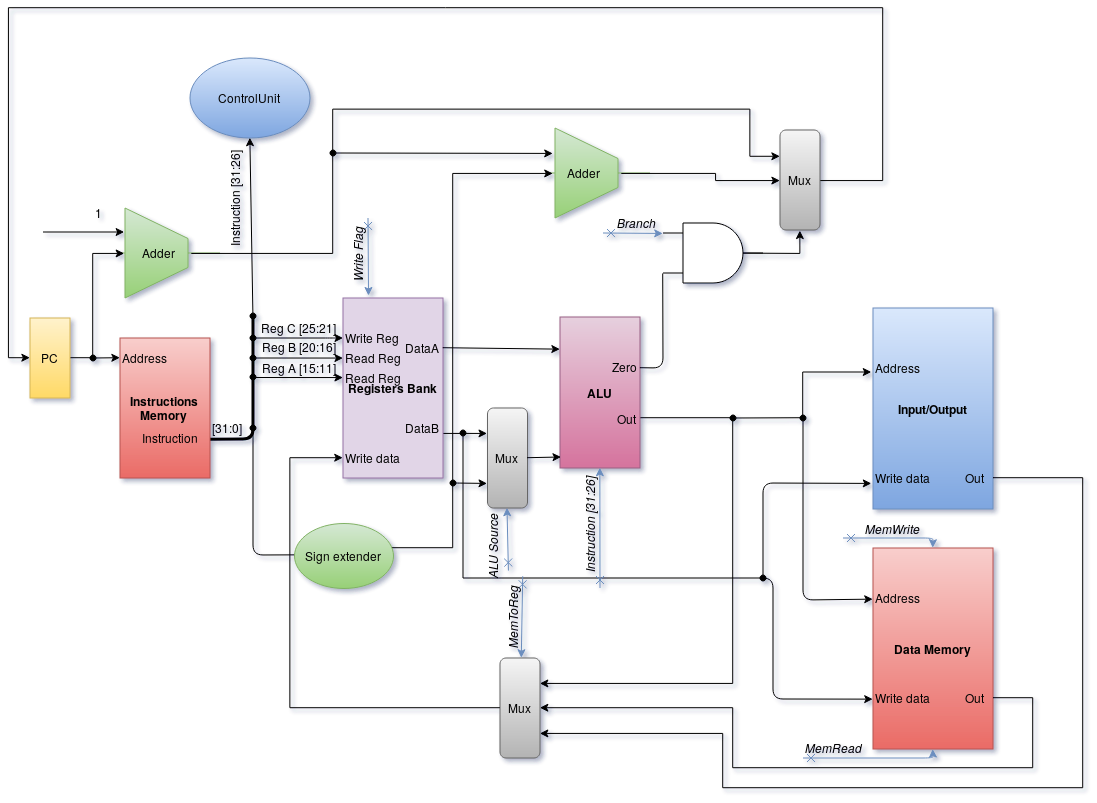
\includegraphics[scale=0.5]{LABAOC.png}
\legend{Fonte: O Autor }
\end{figure}
\end{landscape}

Todos os módulos foram implementados no Quartus II \cite{q2}, utilizando o Verilog.\\

\section{Módulos em Verilog}
Abaixo temos o código fonte do \emph{datapath} do processador e outros módulos que serão importantes para mostrar os resultados.\\
Esse módulo é responsável por instanciar todos os outros módulos e fazer as ligações necessárias entre eles,
além disso ele substitui alguns muxes que estão presentes no esquemático para a
simplificação do processador.\\\\
\textbf{Observação}: Nem todos os sinais são saídas nesse módulo, isso foi feito para a visualização no \emph{Waveform} do Quartus II.

\label{code:main.v}
\lstinputlisting{../../main.v} 

O módulo abaixo é a Memória de Instruções, ela está carregada com seis instruções que são: addi, addi, addi, addi, out e halt.
Isso será importante para a discussão dos resultados.
Ela funciona e foi implementada do mesmo jeito que a Memória de Dados, utilizando o template que o Quartus possui para memórias, 
isso agiliza o tempo de compilação.

\label{code:InstructionsMemory.v}
\lstinputlisting{../../InstructionsMemory/InstructionsMemory.v} 

O módulo abaixo é a Unidade de Controle. O que importa nela é apenas o detalhe da linha 32, onde é utilizado o \emph{negedge clock}. Isso será explicado mais adiante.
Além disso, o que acontece aqui é que para cada tipo de instrução, a Unidade de Controle processa as \emph{flags} corretamente. Essas \emph{flags} são as mostradas na \autoref{fig:esquematico2}.
\label{code:ControlUnit.v}
\lstinputlisting{../../ControlUnit/ControlUnit.v} 

O módulo abaixo é a Unidade Lógica e Aritmética. Ela funciona muito semelhante a Unidade de Controle no quesito de como foi implementada, ambas 
checam para ver qual é a instrução que está sendo executada (através do opcode) e fazem as operações de acordo. A única diferença da Unidade Lógica e Aritmética do CoreBassier para o MIPS é que 
o CoreBassier tem um temporário de 64 bits para verificar se houve \emph{overflow} nas operações.
\label{code:ALU.v}
\lstinputlisting{../../ALU/ALU.v} 

O módulo abaixo é o Banco de Registradores. Não tem nada de especial, é apenas um vetor de posições.
\label{code:RegistersBank.v}
\lstinputlisting{../../RegistersBank/RegistersBank.v} 

O módulo abaixo é a Memória de Dados.
\label{code:DataMemory.v}
\lstinputlisting{../../DataMemory/DataMemory.v} 

O módulo abaixo é a Entrada e Saída.\\
O módulo de Entrada e Saída trata as duas instruções separadamente: ele lê o conjunto de 17 chaves que o kit FPGA possui; e
escreve nos displays de sete segmentos um dado que está no banco de registradores.\\
Quando utiliza-se a instrução de saída, deve-se notar que há como imprimir números separadamente (números de apenas um bit), ou imprimir um conjunto de números,
tudo isso depende de qual é o endereço que foi o alvo da instrução.\\
\label{code:IO.v}
\lstinputlisting{../../IO/IO.v} 


\chapter{Resultados Obtidos e Discussões}
O CoreBassier está completo.\\
Após algumas trocas nas instruções, e no tipo de instruções, está finalizado.
Utilizando as instruções que foram colocadas na Memória de Instruções,
foi realizado o teste utilizando o \emph{Waveform} do Quartus II. 
O código que o processador está rodando é o fibonacci, listado abaixo.

\label{code:fib.asm}
\lstinputlisting{../../InstructionsMemory/fib.asm}

O código funciona da seguinte forma:
Primeiro, é movido 0 para o registrador 2 (que fará o papel de fib[i - 2]) e então
 é movido 1 para o registrador 1 (que fará o papel de fib[i - 1]).
 Após isso é calculado o terceiro termo de fibonacci e iniciado a contagem em 2 (o registrador 5 contará quantos números foram gerados),
 é utilizado a instrução de \textit{input} para obter o valor de parada (ou seja, quantos números de fibonacci o usuário deseja)
 esse valor é armazenado no registador 6.
 Agora começa o laço, com a label L0, onde move-se o conteudo do fib[i - 1] para fib[i - 2], depois o conteudo de fib[i] para fib[i - 1], atualizando os anteriores.
 Então é calculado o próximo valor do fibonacci, somando-se os dois. Com isso, soma-se 1 ao contador \$5, e testa se já foi gerado o número desejado com o \textit{Set on Less Than}.
 E é feito o branch para L0 caso preciso calcular outros valores, ou vai direto para mostrar no display e depois halt, caso não precise.

A \autoref{fig:res1} mostra o primeiro momento após rodado a simulação.\\
A figura detalha todos os sinais, os de controle: branch, branchSignal (controle de desvio), halt (controle de parada), error (erros), overflow (estouro nas operações aritméticas), targetRegister (\emph{flag} para saber qual registrador deve-se escrever), writeRegister (se deve ou não escrever num registrador), 
memoryToRegister (se está a carregar um dado da Memória de Dados para o registrador), memoryWrite (se deve ou não escrever na Memória de Dados), memoryRead (se pode ler a Memória de Dados);
e os intermediários.

\begin{figure}[H]
\centering 
\caption{Antes do primeiro \emph{clock}} \label{fig:res1}
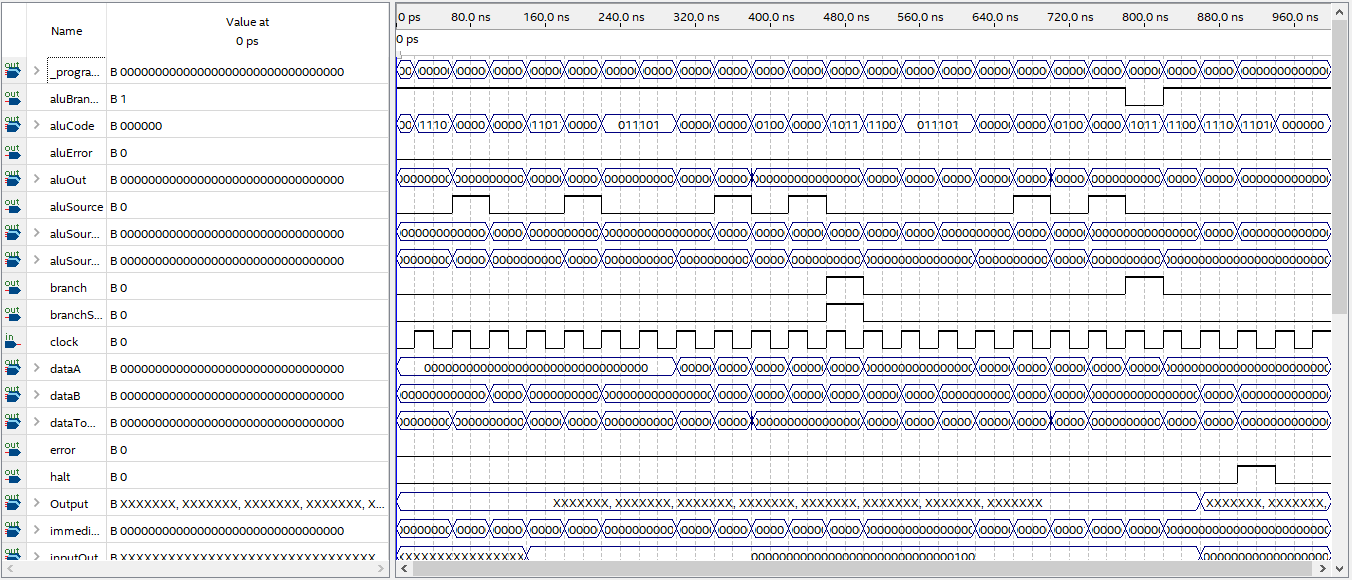
\includegraphics[scale=0.5]{res1.png}
\legend{Fonte: O Autor }
\end{figure}

A \autoref{fig:res2} mostra os sinais após o período de 1 \emph{clock}.\\
A primeira instrução é o mov, então percebe-se que foi buscado o valor de um registrador para passar para o outro.
A Unidade de Controle colocou todos as \emph{flags} para seus valores corretos para ser realizada pela Unidade Lógica e Aritmética a passagem de um para o outro registrador.
\begin{figure}[H]
\centering 
\caption{Resultado do primeiro \emph{clock}} \label{fig:res2}
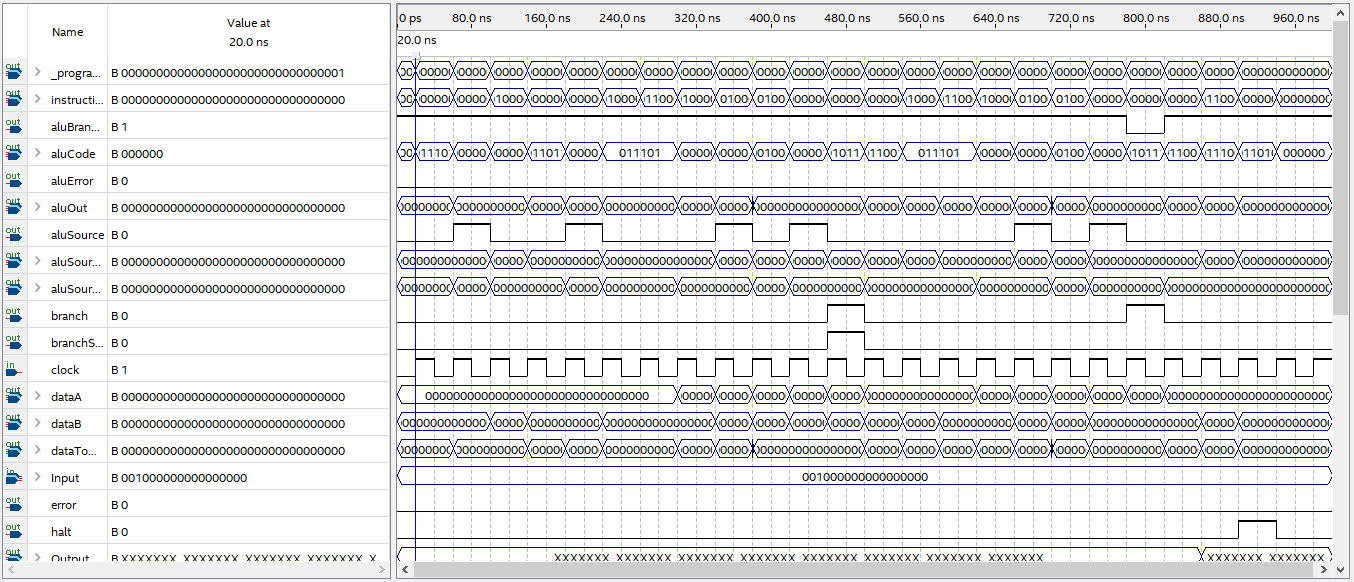
\includegraphics[scale=0.5]{res2.png}
\legend{Fonte: O Autor }
\end{figure}

A \autoref{fig:res3} mostra os sinais após o período de 3 \emph{clock}.\\
A terceira instrução é o add, então percebe-se que foi buscado no banco de registradores.
A Unidade de Controle colocou todos as \emph{flags} para seus valores corretos para a soma ser realizada pela Unidade Lógica e Aritmética e depois ser armazenada 
no registrador 3.\\


\begin{figure}[H]
\centering 
\caption{Resultado do segundo \emph{clock}} \label{fig:res3}
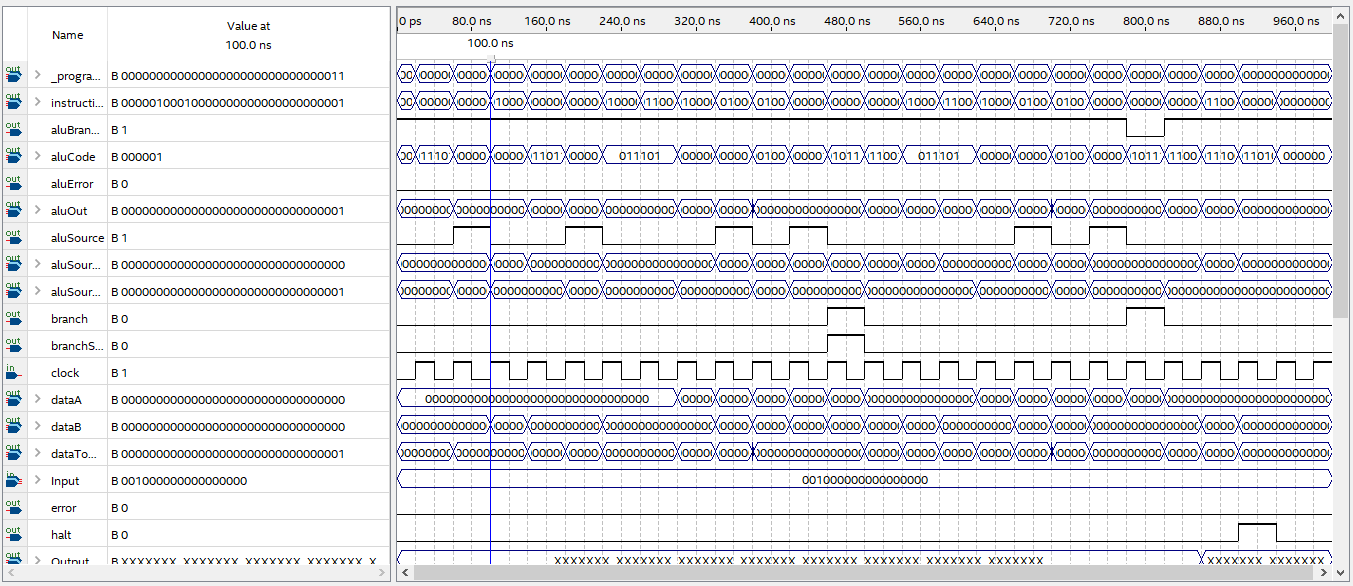
\includegraphics[scale=0.5]{res3.png}
\legend{Fonte: O Autor }
\end{figure}

Isso será repetido mais algumas vezes até chegar na \autoref{fig:res4}.\\
Nesse momento, a instrução sendo executada é o in, e como pode ser visto, o valor $100_2$ é colocado.\\

\begin{figure}[H]
\centering 
\caption{Resultado do último addi} \label{fig:res4}
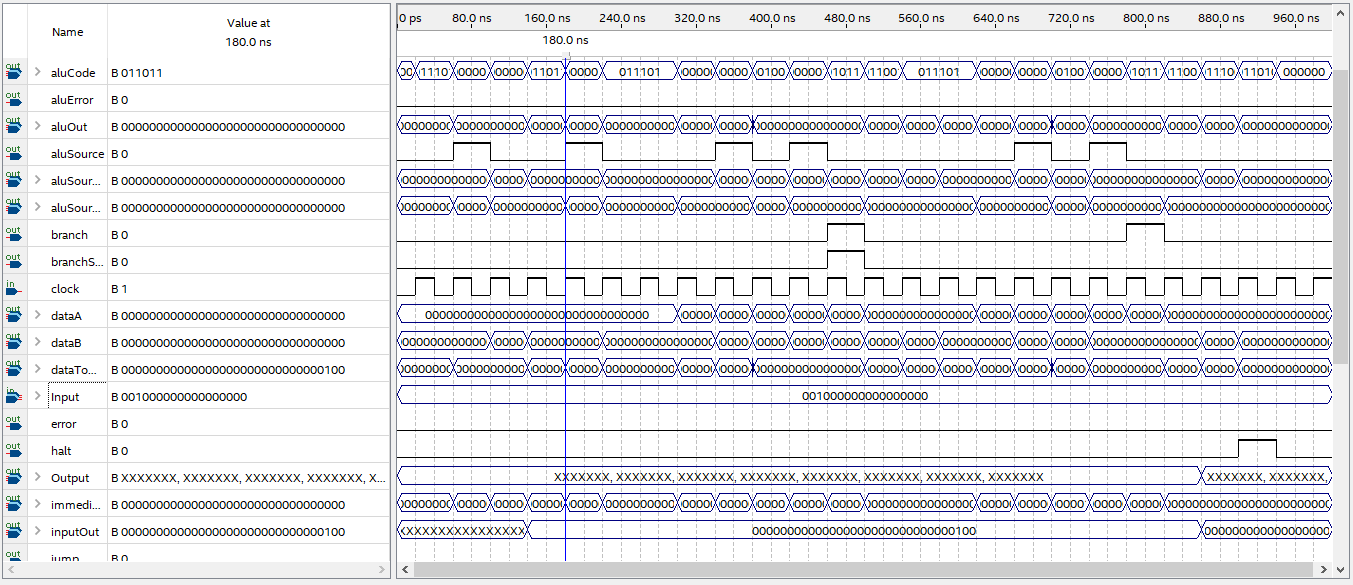
\includegraphics[scale=0.5]{res4.png}
\legend{Fonte: O Autor }
\end{figure}

E por fim, a \autoref{fig:res5} mostra a última instrução que é o halt. Após isso o processador não faz mais nada.
Além disso, pode-se ver que o resultado do programa foi $11_2$ que é o quinto termo: 0 1 1 2 3. (O motivo disso é que o zero é ignorado como primeiro no algoritmo, vide linha 6).

\begin{figure}[H]
\centering 
\caption{Resultado do Halt} \label{fig:res5}
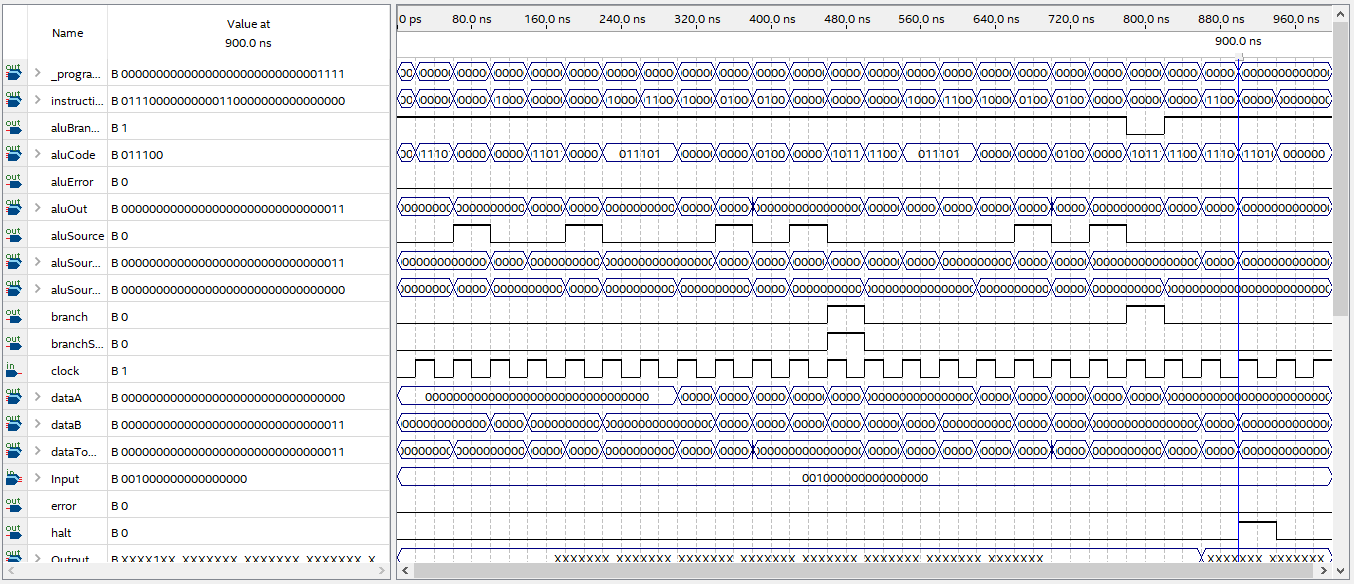
\includegraphics[scale=0.5]{res5.png}
\legend{Fonte: O Autor }
\end{figure}

\chapter{Considerações Finais}
A construção de um processador é um processo muito complexo 
devido as várias considerações de \textit{design} que são 
necessárias. A maior das escolhas é entre seguir a arquitetura 
RISC ou CISC, ambas tem pontos positivos muito interessantes 
(como discutido nas primeiras seções) e que facilitam em algum 
momento da construção do processador. Seja no começo com a 
implementação física dele (no caso do RISC) ou depois, na 
utilização do processador (no caso do CISC).\\
A maior dificuldade encontrada para projetar esse processador foi 
conseguir passar toda a ideia para o Verilog. Ter que pensar nos 
tempos que cada módulo precisa para executar e garantir que o 
\emph{datapath} esteja correto. Por isso foi tão importante os 
\emph{negedge clock}. Isso é uma particularidade do \emph{design} via 
Quartus e Verilog, pois numa implementação física deve-se pensar mais ainda nos tempos -- 
pois no Verilog, uma multiplicação pode durar apenas um \emph{clock}, enquanto
quando é projetado fisicamente, demora muito mais. \\
O próximo passo é arrumar o módulo de IO e fazer o teste na placa FPGA depois 
que tudo estiver pronto. O módulo está implementado, mas ainda não está correto. Além disso, faltam 
outras combinações de instruções para serem testadas. A combinação testada primeiro era apenas somas e um halt,
falta testar \emph{branch} e \emph{load} e \emph{store}.\\
O resultado gerado atendeu as expectativas e objetivo do 
relatório, mostrando como é importante o estudo de arquitetura 
e organização de computadores.


\phantompart
\postextual
\bibliography{referencias}
\phantompart
\printindex
\end{document}
